\input header
\input ras
\def\Koenigs{K\oe nigs }
\font\tencyr=wncyr10
\input cyracc.def
\def\cyr{\tencyr\cyracc}

\footline={\hss\tenrm 6-\folio\hss}\pageno=1

\centerline{\bf LOCAL FIXED POINT THEORY}\bigskip

\centerline{\bf \S6. Attracting and Repelling Fixed Points.}\medskip

Consider a function
$$	f(z)\;=\;\lambda z+a_2 z^2+a_3 z^3+\;\cdots	\eqno (1) $$
which is defined and holomorphic in some neighborhood of the origin, with
a fixed point of multiplier \[\lambda\] at \[z=0\]. If
\[|\lambda|\ne 1\], we will show
that \[f\] can be reduced to a simple normal form by a suitable change of
coordinates. First consider the case \[\lambda\ne 0\],
so that the origin is not a critical point. The following was proved by G.
\Koenigs in 1884.

{\QP{\bf 6.1. \Koenigs Linearization Theorem.} {\it If the
 multiplier \[\lambda\] satisfies\break \[|\lambda|
 \ne 0, 1\], then there exists a local holomorphic change of coordinate
 \[w=\phi(z)\], with \[\phi(0)=0\], so that \[\;\phi\circ\! f\!\circ
 \phi^{-1}\,\] is the linear
 map \[w\mapsto\lambda w\] for all \[w\] in some neighborhood of the origin.
 Furthermore, \[\phi\] is unique up to multiplication by a non-zero constant.
 }\medskip}

\noindent (This functional equation \[\,\phi\circ\! f\!\circ
 \phi^{-1}(w)\,=\,\lambda w\,\] had been studied some years earlier by
 Schr\"oder, who believed however that it did not have many solutions.)
\smallskip

 {\bf Proof of uniqueness.} If there were two such maps \[\phi\] and \[\psi\],
 then the composition
 $$	\psi\circ\phi^{-1}(w) \;=\;b_1 w+ b_2 w^2+b_3 w^3+\,\cdots	$$
 would commute with the map \[w\mapsto\lambda w\]. Comparing coefficients
 of the two resulting power series, we see that \[\lambda b_n=b_n\lambda^n\]
 for all \[n\]. Since \[\lambda\] is neither zero nor a root of unity,
 this implies that
 \[b_2=b_3=\cdots=0\]. Thus \[\psi\circ\phi^{-1}(w) \;=\;b_1 w\], or in
 other words \[\psi(z)=b_1\phi(z)\].\smallskip

 {\bf Proof of existence when \[0<|\lambda|<1\].} Choose a constant \[c<1\]
 so that\break
 \[c^2<|\lambda|<c\], and choose a neighborhood \[D_r\] of the origin
 so that \[|f(z)|\le c|z|\] for \[z\in D_r\]. Thus for any starting point
 \[z_0\in D_r\], the orbit \[z_0\mapsto z_1\mapsto\cdots\] under \[f\]
 converges geometrically towards the origin, with \[|z_n|\le rc^n\].
 By Taylor's Theorem,
 $$	|f(z) - \lambda z| \;\le\; k|z^2|	$$
 for some constant \[k\] and for all \[z\in D_r\], hence
 $$	|z_{n+1}-\lambda z_n|\;\le\; kr^2 c^{2n}\,.	$$
 It follows that the numbers \[w_n=z_n/\lambda^n\] satisfy
 $$	|w_{n+1}- w_n|\;\le\; k'(c^2/|\lambda|)^n\,,	$$
 where \[k'=kr^2/|\lambda|\]. These differences converge
 uniformly and geometrically to zero.\break\eject
 \noindent Thus the holomorphic
 functions \[z_0\mapsto w_n(z_0)\] converge, uniformly throughout \[D_r\],
 to a holomorphic limit \[\;\phi(z_0)\,=\,\lim_{n\to\infty}\; z_n/\lambda^n\].
 The required identity \[\;\phi(f(z))\;=\;\lambda\phi(z)\]\break follows
 immediately. A similar argument shows that \[|\phi(z)-z|\] is less than or
 equal to some constant times \[|z^2|\]. Therefore \[\phi\] has derivative
 \[\phi'(0)=1\], and hence is a local conformal diffeomorphism.

 {\bf Proof when \[|\lambda|>1\].} Since \[\lambda\ne 0\], the inverse
 map \[f^{-1}\] is locally well defined and holomorphic, having the origin as
 an attractive fixed point with multiplier \[\lambda^{-1}\]. Applying the
 above argument to \[f^{-1}\], the conclusion follows.\QED

{\bf 6.2. Remark.} More generally, suppose that we consider a
family of maps \[f_\alpha\] of the form (1) which depend holomorphically on
one (or more) complex parameters
\[\alpha\] and have multiplier \[\lambda=\lambda(\alpha)\]
satisfying \[|\lambda(\alpha)|\ne 0,\,1\]. Then
a similar argument shows that {\it the \Koenigs
 function \[\phi(z)=\phi_\alpha(z)\] depends holomorphically on
\[\alpha\].}  This fact will be important in \S8.5.
To prove this statement, let us fix \[0<c<1\]
 and suppose that \[|\lambda(\alpha)|\] varies
through some compact subset of the interval
 \[(c^2,\,c)\]. Then it is easy to check that the convergence in the proof
 of 6.1 is uniform in \[\alpha\]. The conclusion now follows easily.\QED
\smallskip

 {\bf 6.3. Remark.} The \Koenigs Theorem helps us to understand
 why the Julia set \[J(f)\] is so often a complicated ``fractal" set.
 {\it Suppose that there exists a single repelling periodic point \[\hat z\]
 for which
 the multiplier \[\lambda\] is not a real number. Then \[J(f)\] cannot
 be a smooth manifold, unless it is all of \[\hat\C\].} To see this,
 choose any point \[z_0\in J(f)\] which is close to \[\hat z\], and let
 \[w_0=\phi(z_0)\]. Then \[J(f)\] must also contain an infinite sequence
 of points \[z_1\,,\,z_2\,,\,\ldots\] with \Koenigs coordinates \[\;\phi(z_n)
 =w_n/\lambda^n\;\] which lie along a logarithmic spiral and converge to zero.
 Evidently such a set can not lie in any smooth submanifold of \[\C\].
 Furthermore, if we recall that the iterated pre-images of our fixed
 point are everywhere dense in \[J(f)\], then we see that such sequences
 lying on logarithmic spirals are extremely pervasive. Compare Figures 3
 and 4 which show typical examples of such spiral structures, associated with
 repelling points of periods 2 and 1 respectively.\smallskip

 We can restate 6.1 in a more global form as follows.

 {\QP {\bf 6.4. Corollary.} {\it Suppose that \[f:S\to S\] is a holomorphic
 map from a Riemann surface to itself with an attractive fixed point of
 multiplier \[\lambda\ne 0\] at \[\hat z\].
 Let \[\Omega\subset S\] be the basin of attraction,
 consisting of all \[z\in S\] for which \[\lim_{n\to\infty}\;
 f^{\circ n}(z)\] exists and is equal to \[\hat z\].
 Then there is a holomorphic map \[\phi\] from \[\Omega\] onto \[\C\] so that
 the diagram
 $$	\matrix{\Omega& \buildrel f\over\longrightarrow & \Omega\cr
	 \quad\downarrow\phi & & \quad\downarrow\phi\cr
	 \C&\buildrel \lambda{\textstyle\cdot}\over\longrightarrow &\;\C\cr}
	 \eqno (2) $$
 is commutative, and so that \[\phi\] takes a neighborhood of \[\hat z\]
 diffeomorphically onto a neighborhood of zero.
 Furthermore, \[\phi\] is unique up to multiplication
 by a\break constant.}\medskip}

 \noindent In fact, to compute \[\phi(z_0)\] at an arbitrary point of \[\Omega\]
 we must simply follow the orbit
 of \[z_0\] until we reach some point \[z_n\] which is very close to
 \[\hat z\], then evaluate the \Koenigs coordinate
 \[\phi(z_n)\] and multiply by \[\lambda^{-n}\].\QED\eject

 \pageinsert
 \vfil %\endinsert

% \pageinsert\vfil
 \insertRaster qj_spir.ps pixels 960 by 720 scaled 310
 \smallskip
 \centerline{Figure 3. Detail of Julia set for \[z\mapsto z^2-.744336+.121198i\].}
 \bigskip
 \insertRaster qj_mis.ps pixels 720 by 990 scaled 320
 \smallskip
 \centerline{Figure 4. Detail of Julia set for
 \[z\mapsto z^2+.424513+.207530i\].}
 \vfil\endinsert

 As an example, Figure 5 illustrates the map
 \[f(z)= z^2+0.7z\]. Here the Julia set \[J\] is the outer Jordan curve,
 bounding the basin \[\Omega\] of the attracting fixed point.
 The critical point \[\omega=-0.35\]
 is at the center of the picture, and the attracting fixed point \[\hat z=0\]
 is directly above it.
 The curves \[\;|\phi(z)|={\rm constant}=|\phi(\omega)/\lambda^n|\;\] have
 been drawn in.
 Note that \[\phi\] has zeros at all iterated preimages of \[\hat z\],
 and critical points at all iterated preimages of the critical point \[\omega\].
 The function \[z\mapsto\phi(z)\] is unbounded, and oscillates wildly as
 \[z\] tends to \[J=\partial\Omega\].\medskip

 \pageinsert\vfil
 \insertRaster qj_phi.ps pixels 960 by 960 scaled 400
 \bigskip\bigskip
 \centerline{Figure 5. Julia set for \[z\mapsto z^2+.7z\], with curves
 \[|\phi|={\rm constant}\].}
 \vfil\endinsert

 The statement is the repelling case is somewhat different:

 {\QP{\bf 6.5. Corollary.} {\it If
 \[\hat z\] is a repelling fixed point, then there
 is a holomorphic map \[\psi:\C\to S\] in the opposite direction,
 so that the diagram
 $$      \matrix{S& \buildrel f\over\longrightarrow & S\cr
	 \quad\uparrow\psi & & \quad\uparrow\psi\cr
	 \C&\buildrel \lambda{\textstyle\cdot}\over\longrightarrow &\C\cr}   $$
 is commutative, and so that \[\psi\] maps a neighborhood of zero
 diffeomorphically onto a neighborhood of \[\hat z\]. Here
 \[\psi\] is unique except that it may be replaced by \[w\mapsto
 \psi(cw)\] for any constant \[c\ne 0\].}\medskip}

 To compute \[\psi(w)\] we simply choose some \[\lambda^{-n}w\] which
 is so small that \[\phi^{-1}(\lambda^{-n}w)\] is defined, and then
 apply \[f^{\circ n}\] to the result.\QED\smallskip

 Now suppose that \[f:\hat\C\to\hat\C\] is a rational function with an
 attracting fixed point \[\hat z\].
 By the {\bit immediate basin} \[\Omega_0(\hat z)\]
 we mean the connected component of \[\hat z\] in the
 basin of attraction \[\Omega=\Omega(\hat z)\], or equivalently the
 connected component of \[\hat z\] in the Fatou set \[\hat\C\ssm J\].
 (Compare 4.3.) The following is due to Fatou and Julia.

 {\QP{\bf 6.6. Theorem.} \it If \[f\] has degree two or more,
 then the immediate basin of any attracting fixed point \[\hat z\] of \[f\]
 contains at least one critical point.
 Furthermore, if the multiplier \[\lambda\] is not zero, then there exists a
 unique compact neighborhood \[\bar U\] of \[\hat z\] in \[\Omega_0\] which:

 \noindent $(a)$ maps bijectively onto some round disk \[\bar D_r\] under the
 \Koenigs map \[\phi\], and

 \noindent $(b)$ has at least one critical point on its boundary \[\partial U\].
 \medskip}

 \noindent Evidently \[\bar U\] can be described as
 the largest neighborhood which maps bijectively to
 a round disk centered at the origin. As an example, in Figure 5 the region
 \[U\] is bounded by the top half of the central figure 8 shaped curve.
 \smallskip

 {\bf Proof of 6.6.} If \[\lambda=0\], then \[\hat z\] itself is critical.
 Thus we may
 assume that \[\lambda\ne 0\] and apply 6.1. Evidently some branch
 \[\phi_0^{-1}\] of the inverse map
 can be defined as a single valued holomorphic function over some small disk
 \[D_\epsilon\], with \[\phi_0^{-1}(0)=\hat z\]. Let us try to extend
 \[\phi_0^{-1}\] by analytic continuation along radial lines through the
 origin in \[D_\epsilon\]. It cannot be possible to extend indefinitely far in
 every direction; for then \[\phi_0^{-1}\] would be a non-constant holomorphic
 map from the entire plane \[\C\] into the basin \[\Omega_0(\hat z)\]. This
 is impossible, since this basin is Hyperbolic.
 Thus there must exist some largest
 radius \[r\] so that \[\phi_0^{-1}\] extends analytically throughout the open
 disk \[D_r\]. Let \[U=\phi_0^{-1}(D_r)\]. We must prove that the closure
 \[\bar U\] is a compact subset of the basin
 \[\Omega(\hat z)\], and also that there is at least one critical point of \[f\]
 on the boundary \[\partial U\].
 If \[z_1\in\partial U\] is any boundary point, then
 using the identity \[\phi(f(z))=\lambda\phi(z)\in D_{|\lambda|r}\] for \[z\in U\]
 arbitrarily close to \[z_1\], we see that \[f(z_1)\] belongs to the open
 set \[U\subset \Omega\]. Therefore \[z_1\] also belongs to the basin
 \[\Omega\], with \[|\phi(z_1)|=r\] by continuity.
 Now at least one such \[z_1\] must be a critical
 point of \[f\]. For whenever \[z_1\] is non-critical we can continue
 \[\phi_0^{-1}\] analytically throughout a neighborhood of the image point
 \[\phi(z_1)\in\partial D_r\] simply by chasing around Diagram (2),
 composing the map \[z\mapsto
 \phi_0^{-1}(\lambda z)\] with the branch of \[f^{-1}\] which carries \[f(z_1)\]
 to \[z_1\].\QED

 For further information about the attractive basin \[\Omega_0\] see \S13.4,
 and also \S17.1.\medskip

 Next let us consider the {\bit superattracting} case \[\lambda=0\]. The
 following was proved by B\"ottcher in 1904.\smallskip

{\bf Historical Note:} L. E. B\"ottcher was born in Warsaw in 1872. He
took his doctorate in Leipzig in 1898, working in Iteration Theory, and
then moved to Lvov. He published in Polish and Russian. (The Russian form
of his name is ~{\cyr B\"etkher\cdprime}$\, $.)

 {\QP {\bf 6.7. Theorem of B\"ottcher.} {\it Suppose that
 $$	f(z)\;=\;a_nz^n\,+\,a_{n+1}z^{n+1}\,+\,\cdots\;,	$$
 where \[n\ge 2\], \[a_n\ne 0\]. Then there exists a local
 holomorphic change of coordinate \[w=\phi(z)\] which conjugates \[f\] to the
 \[n$-th power map \[\;w\mapsto w^n\;\]
 throughout some neighborhood
 of \[\phi(0)=0\]. Furthermore, \[\phi\] is unique up to multiplication by
 an \[(n-1)$-st root of unity.}\medskip}

 Thus near any critical fixed point, \[f\] is conjugate to a map of the form
 $$	\phi\circ f\circ\phi^{-1}\,:\,w\;\mapsto\;w^n\,,	$$ 
 with \[n\ne 1\]. This Theorem is most often applied in
 the case of a fixed point at infinity. For example, any polynomial
 map \[p(z) =a_nz^n+a_{n-1}z^{n-1}+\cdots+ a_0\] of degree \[n\ge 2\] has
 a superattractive fixed point at infinity. It follows easily from 6.7
 that there is a
 local holomorphic map \[\psi\] taking infinity to infinity which conjugates
 \[p\] to the map \[w\mapsto w^n\] around \[w=\infty\].\smallskip

 The proof is quite similar to the \Koenigs proof. It is only
 necessary to first make a logarithmic change of coordinates, and to be
 careful since the logarithm is not a single valued function. Suppose, to fix
 our ideas, that we consider a map having a fixed point at infinity,
 with a Laurent series expansion of the form
 $$	f(z)\; =\;a_nz^n+a_{n-1}z^{n-1}+\cdots+a_0+a_{-1}z^{-1}+\cdots $$
 with \[n\ge 2\],
 convergent for \[|z|>r\]. Note first that the linearly conjugate map\break
 \[z\mapsto \alpha f(z/\alpha)\], where \[\alpha^{n-1}=a_n\], has leading
 coefficient equal to \[+1\]. Thus, without loss of generality, we may
 assume that \[f\] itself has leading coefficient \[a_n=1\].
 Then\break \[f(z)=z^n(1+{\cal O}|1/z|)\] for \[|z|\] large,
 where \[{\cal O}|1/z|\] stands for some expression which is bounded by a
 constant times \[|1/z|\].
 Let us make the substitution \[z=e^Z\], where \[Z\]
 ranges over the half-plane \[{\cal R}(Z)>\log(r)\]. Then \[f\] lifts to
 a continuous map
 $$	F(Z)=\log f(e^Z)\;,	$$
 which is uniquely
 defined up to addition of some multiple of \[2\pi i\]. With correct choice of
 this lifting \[F\], it is not hard to check that
 \[\;F(Z)\;= \;nZ+{\cal O}(e^{-{\cal R}(Z)})\;\]
 for \[{\cal R}(Z)\] large. In fact, we will only need the weaker
 statement that
 $$	|F(Z)-nZ|<1	\eqno (3)	$$
 for \[{\cal R}(Z)\] large. Let us choose \[\sigma>1\] to be large enough
 so that the inequality (3) is satisfied for all \[Z\] in the half-plane
 \[{\cal R}(Z)>\sigma\]; note that \[F\] necessarily maps this half-plane
 into itself. Note the identity
 \[F(Z+2\pi i)=F(Z)+2\pi in\], which follows since \[F(Z+2\pi i)-F(Z)\]
 is a multiple of \[2\pi i\] which differs from \[n(Z+2\pi i)-nZ\] by at most
 2. If \[Z_0\mapsto
 Z_1\mapsto\cdots\] is any orbit under \[F\] in this half-plane, then we have
 \[|Z_{k+1}-nZ_k|<1\]. Setting \[W_k=Z_k/n^k\], it follows that
 $$	|W_{k+1}-W_k|<1/n^{k+1}	\,. $$
 Thus the sequence of holomorphic functions \[W_k=W_k(Z_0)\] converges
 uniformly and geometrically as \[k\to\infty\] to a holomorphic limit
 \[\Phi(Z_0)=\lim_{k\to\infty}\; W_k(Z_0)\].
 Evidently this mapping \[\Phi\] satisfies the identity
 $$	\Phi(F(Z))\;=\;n\Phi(Z)\,.	$$
 Note also that \[\Phi(Z+2\pi i)=\Phi(Z)+2\pi i\]. Therefore the mapping
 \[\phi(z)=\exp(\Phi(\log z))\] is well defined near infinity, and
 satisfies the required identity \[\phi(f(z))=\phi(z)^n\].

 To prove uniqueness, it suffices to study mappings \[w\mapsto \eta(w)\]
 near infinity which satisfy \[\eta(w^n)=\eta(w)^n\]. Setting \[
 \;\eta(w)= c_1w+c_0+c_{-1}w^{-1}+\cdots\;,	\]
 this becomes
 $$	c_1w^n+c_0+c_{-1}w^{-n}+\cdots\;=\; (c_1w+c_0+\cdots)^n\;=\;
	 c_1^nw^n+nc_1^{n-1}c_0w^{n-1}+\cdots\,.	$$
 Since \[c_1\ne 0\], \[c_1\] must be an \[(n-1)$-st root of unity,
 and an easy induction shows that the remaining coefficients are zero.\QED
 \smallskip

 {\bf Caution.} In analogy with 6.4, one might hope that the change of
 coordinates\break \[z\mapsto\phi(z)\] extends throughout the entire basin
 of attraction of the superattractive point as a holomorphic mapping.
 (Compare \S17.3.) However, this is not always possible. Such an extension
 involves computing expressions of the form
 $$	z\mapsto \root n \of {\phi(f(z))}\;,	$$
 and this does not work in general since the \[n$-th root cannot be
 defined as a single valued function. For example, there is trouble
 whenever some other point in the basin maps exactly onto the superattractive
 point, or whenever the basin is not simply-connected.\smallskip

 We conclude with a problem.
 \lln

 {\bf Problem 6-1.} What maps to what in Figure 5?
 \vfil
\eject

\footline={\hss\tenrm 7-\folio\hss}\pageno=1


 \centerline{\bf \S7. Parabolic Fixed Points: the Leau-Fatou Flower.}
 \medskip

 Again we consider functions \[\;   f(z)\;=\;\lambda z+a_2 z^2+a_3 z^3+\;
 \cdots    \;\]
 which are defined and holomorphic in some neighborhood of the origin,
 but in this section
 we suppose that the multiplier \[\lambda\] at the fixed point
 is a root of unity, \[\lambda^q=1\]. Such a fixed point
 is said to be {\bit parabolic}, provided that \[f^{\circ q}\] is not the
identity map. (More generally, any periodic orbit
 with \[\lambda\] a root of unity is called parabolic, provided that no
iterate of \[f\] is the identity map.) First consider
 the special case
 \[\lambda=1\]. It will be convenient to write our map as
 $$	f(z)\;=\;z+az^{n+1}+\,({\rm higher\;terms})\,,	\eqno (7.1) $$
 with \[a\ne 0\]. The integer
 \[n+1\ge 2\] is called the {\bit multiplicity}$\,$ of the fixed point.
 (By definition, the `` simple" fixed points with \[\lambda\ne 1\] have
 multiplicity equal to 1.) Choose a neighborhood \[N\]
 of the origin which is small enough so that \[f\] maps \[N\]
 diffeomorphically onto some neighborhood \[N'\] of the origin.\smallskip

 {\bf Definition.} A connected open set \[U\],
 with compact closure \[\bar U\subset N\cap N'\], will be called an
 {\bit attracting petal}$\,$ for \[f\] at the origin if
 $$	f(\bar U)\subset U\cup\{0\}\qquad{\rm and}\qquad
	 \bigcap_{k\ge 0}\;f^{\circ k}(\bar U)=\{0\}\,.	$$
 Similarly, \[U'\subset N\cap N'\] is a {\bit repelling petal}$\,$ for \[f\]
 if \[U'\] is an attracting petal for \[f^{-1}\].\smallskip

 {\QP{\bf 7.2. Leau-Fatou Flower Theorem.} {\it If the origin is a fixed
 point of multiplicity \[n+1\ge 2\], then there exist \[n\] disjoint
 attracting petals \[U_i\] and \[n\] disjoint repelling petals \[U'_i\] so
 that the union of these \[2n\] petals, together with the origin itself,
 forms a neighborhood \[N_0\] of the origin. These petals
 alternate with each other, as illustrated in Figure 6, so
 that each \[U_i\] intersects only \[U'_i\] and \[U'_{i-1}\] $($where
 \[U'_0\] is to be identified with \[U'_n\,)\].}\medskip}

 If \[U_i\] is an attracting petal, then evidently
 the sequence of maps \[f^{\circ k}\] restricted to \[\bar U_i\]
 converges uniformly to zero.
 On the other hand, if \[U_i'\] is a repelling
 petal, then every orbit \[z_0\mapsto z_1\mapsto\cdots\] which starts out in
 \[U_i'\] must eventually leave \[U_i'\], and in fact must leave the union
 \[U_1'\cup\cdots\cup U_n'\]. (However it may later return, perhaps
 even infinitely often.) Here are three immediate consequences of 7.2.

 {\QP{\bf 7.3. Corollary.} {\it There is no periodic orbit,
 other than the fixed point at the origin, which is
 completely contained within the neighborhood \[N_0\].}\medskip}

 \pageinsert
\insertRaster flower.ps pixels 640 by 480 scaled 500
\smallskip
 \centerline{Figure 6. Leau-Fatou Flower with three attracting}
\centerline{ petals \[U_i\] and three repelling petals \[U'_i\].}
\bigskip
\insertRaster fig7.ps pixels 640 by 480 scaled 550
 \centerline{Figure 7.}\bigskip
 \endinsert

 Now suppose that \[f\] is a globally defined rational function. We continue
 to assume that the origin is a fixed point with \[\lambda=1\].
 Each attracting petal \[U_i\] determines a parabolic {\bit basin of attraction}
 \[\Omega_i\], consists of all \[z_0\] for which the orbit
 \[z_0\mapsto z_1\mapsto\cdots\] eventually lands in the attracting
 petal \[U_i\], and hence converges to the fixed point through \[U_i\].
 Evidently these basins \[\Omega_1\,,\,\ldots\,,\, \Omega_n\] are disjoint open
 sets.

 {\QP {\bf 7.4 Corollary.} {\it If we exclude the case of an orbit
 which exactly hits the fixed point, 
 then an orbit \[z_0\mapsto z_1\mapsto\cdots\] under \[f\] converges to
 the fixed point if and only if it eventually
 lands in one of the attracting petals \[U_i\], and hence belongs to
 the associated basin \[\Omega_i\].}\medskip}
 \eject % ???
 % \advancepageno

 {\QP{\bf 7.5. Corollary.} {\it Each parabolic
 basin \[\Omega_i\] is contained in
 the Fatou set \[\hat\C\ssm J(f)\], but each basin boundary \[\partial \Omega_i\]
 is contained in the Julia set \[J(f)\].
 It follows that each repelling petal \[U'_i\] must intersect
 \[J(f)\].}\medskip}

 \noindent In particular, it is claimed
 that the parabolic fixed point \[z=0\] must
 belong to \[J(f)\].\smallskip

 {\bf Proof of 7.5.} We first show that \[0\in
 J(f)\]. It follows from 7.1 that
 $$	f^{\circ k}(z)\;=\; z+kaz^{n+1}+{\rm (higher\;terms)}\,. $$
 Evidently no sequence of iterates \[f^{\circ k}\] can converge uniformly
 in a neighborhood of the origin, since the corresponding
 \[(n+1)$-st derivatives do not converge. (Compare 1.3.)
 Thus \[0\in J(f)\], and it follows
 that every point in the grand orbit of zero belongs to \[J(f)\].
 If \[z_1\in\partial \Omega_i\] is not in the grand orbit of zero,
 then by 7.4 we can extract
 a subsequence from the orbit of \[z_1\] which remains bounded away from
 zero. Since the sequence of iterates \[f^{\circ k}\] converges to zero
 throughout the open set \[\Omega_i\], it follows that \[\{f^{\circ k}\}\] can not
 be normal in any neighborhood of the boundary point \[z_1\]. The proof
 is now straightforward.\QED\medskip

 {\bf Proof of Theorem 7.2.} We will say that a vector \[v\in\C\] points in
 an {\bit attracting direction} at the fixed point of 7.1 if
 the product \[av^n\] is
 real and negative. If we ignore higher order terms, then these are just the
 directions for which the vector from \[v\] to \[f(v)\approx v(1+av^n)\]
 points straight in towards the origin. Similarly, \[v\] points in
 a {\bit repelling
 direction} if \[av^n\] is real and positive.
 Evidently there are \[n\] equally spaced attracting directions which are
 separated by the \[n\] equally spaced repelling directions.

 We will make use of the substitution \[w=b/z^n\] with inverse
 \[z=\root n \of {b/w}\], where \[b=-1/(na)\].
 Evidently the sector between two repelling
 directions in the \[z$-plane will correspond under this transformation
 to the entire \[w$-plane, slit along the negative real axis. In particular,
 a neighborhood of zero in such a sector will correspond to a neighborhood
 of infinity in such a slit \[w$-plane. Let us write the transformation
 7.1 as
 $$	z\mapsto f(z)=z(1+az^n+o|z^n|)	$$
 as \[|z|\to 0\]. Here \[o|z^n|\] stands for a remainder term whose ratio
 to \[|z^n|\] tends to zero.
 Substituting \[z=(b/w)^{1/n}\], the corresponding
 self-transformation in the \[w$-plane is
 $$	w\mapsto w'\;=\;b/f(z)^n\;=\;(b/z^n)(1+az^n+o|z^n|)^{-n}\;=\;
	 w(1-naz^n+o|z^n|)	\,.	$$
 But \[z^n=b/w\] and \[nab=-1\], so this can be written simply as
 $$	w'\;=\; w(1+w^{-1}+o|w^{-1}|)\;=\; w+1+o(1)	$$
 as \[|w|\to\infty\]. In other words, given any small number, which it will
 be convenient to write as \[\sin\epsilon>0\], we can choose a radius \[r\]
 so that
 $$	|w'-w-1|<\sin\epsilon\quad{\rm for}\quad |w|>r\,.	$$
 It follows that the slope of the vector from \[w\] to \[w'\] satisfies
 \[\;|{\rm slope}|<\tan
 \epsilon\,\], as long as \[|w|>r\]. Now we can construct an ``attracting
 petal for the point at infinity'' in the \[w$-plane as follows.
 Let \[P\]
 consist of all \[w=u+iv\] with \[|w|>r\], and with \[u>c-|v|/\tan 2\epsilon\],
 where the constant \[c\] is large enough so that all points \[w\in P\]
 satisfy \[|w|>r\]. (Figure 7.) Then an easy geometric argument shows that
 the closure \[\bar P\] is mapped into \[P\], and that every backward orbit
 starting in \[\bar P\] must eventually leave \[\bar P\]. Translating
 these statements back to the \[z$-plane, the proof can easily be
 completed.\QED

 Now suppose that the multiplier \[\lambda\] is a \[q$-th root of unity,
 say \[\lambda=\exp(2\pi ip/q)\] where \[p/q\] is a fraction in lowest
 terms. Then we can apply the discussion above to the \[q$-fold iterate
 \[f^{\circ q}\].

 {\QP{\bf 7.6. Lemma.} {\it If the multiplier \[\lambda\] at a fixed point
 \[f(z_0)=z_0\] is a primitive \[q$-th root of unity, then the 
 number \[n\] of attractive petals around \[z_0\] must be a multiple of \[q\].
 In other words, the
 multiplicity \[n+1\] of \[z_0\] as a fixed point of
 \[f^{\circ q}\] must be congruent to 1 modulo \[q\].}\medskip}

 Intuitively, if we perturb \[f\] so as to change \[\lambda\] slightly, then
 the multiple fixed point of \[f^{\circ q}\] will split up into one
 point which is still fixed by \[f\] together with some finite collection
 of orbits which have period \[q\] under \[f\]. This Lemma can be proved
 geometrically by showing that multiplication by \[\lambda=f'(z_0)\] must
 permute the \[n\] attractive directions at \[z_0\]. It can be proved
 by a formal power series computation based on the observation that
 \[f\circ f^{\circ q}\;=\;f^{\circ q}\circ f\]. Details will be left to
 the reader.\QED
 % \eject
 % \pageno=33

 As an example, Figure 8 shows part of the Julia set for the polynomial
 \[z\mapsto z^2+\lambda z\] where \[\lambda\] is a seventh root of unity,
 \[\lambda=e^{2\pi it}\] with \[t=3/7\]. There are seven attractive petals
 about the origin.\medskip

 We can further describe the geometry around a parabolic
 fixed point as follows.
 As in 7.1, we consider a local analytic map with a fixed point
 of multiplier \[\lambda=1\]. Let \[U\]
 be either one of the \[n\] attracting petals or one of the \[n\]
 repelling petals, as described in the Flower Theorem, \S7.2.
 Form an identification space \[U/f\] from \[U\] by identifying \[z\]
 with \[f(z)\] whenever both \[z\] and \[f(z)\] belong to \[U\]. (This
 means that \[z\] is identified with \[f(z)\]
 for every \[z\in U\] in the case of an attracting petal,
 and for every \[z\in U\cap f^{-1}(U)\] in the case of a repelling petal.)
 By definition, a holomorphic map \[\alpha:U\to\C\] is {\bit univalent}
 if distinct points of \[U\] correspond to distinct points of \[\C\].
 The following was proved by Leau and Fatou.
 \midinsert
 \vfil
 \insertRaster qj_3over7.ps pixels 1008 by 816 scaled 350
 \bigskip\bigskip
 \centerline
 {Figure 8. Julia set for \[z\mapsto z^2+e^{2\pi it}z\] with \[t=3/7\].}
 \vfil\endinsert

 {\QP{\bf 7.7. Theorem.} {\it The quotient manifold \[U/f\] is conformally
 isomorphic to the infinite cylinder \[\C/\Z\]. Hence there is one, and
 up to composition with a translation only one, univalent embedding \[\alpha\]
 from \[U\] into the universal covering space \[\C\] which satisfies the
 {\bit Abel functional equation}
 $$	\alpha(f(z))\;=\;1+\alpha(z)	$$
 for all \[z\in U\cap f^{-1}(U)\]. With suitable choice of \[U\], the image
 \[\alpha(U)\subset \C\] will contain
 some right half-plane \[\{w:{\cal R}(w)>c\}\] in the case of an attracting
 petal, or some left half-plane in the case of a repelling petal.}\medskip}

 By definition, the quotient \[U/f\] is called an {\bit \'Ecalle cylinder}
 for \[U\]. (This term is due to Douady, suggested by the work of \'Ecalle
 on holomorphic maps tangent to the identity.)\smallskip
 % \eject
 % \advancepageno

 The proof of 7.7 begins as follows.
 To fix our ideas, we consider only the case of an
 attracting petal. As in the proof of 7.2, a substitution of the form
 \[w=b/z^n\] will conjugate the map \[f\] of \S7.1 to a map
 which has the form
 $$	 g(w)\;=\; w + 1 + a_1 w^{-1/n} + a_2 w^{-2/n}+\,\cdots\;. $$
 Here \[w\] ranges over a neighborhood of infinity, with the negative
 real axis removed.\smallskip

 {\bf Definition.} Let \[{\cal G}\] be the group
 consisting of all holomorphic maps which are defined and univalent in
 some region of the form
 $$ \{\;u+iv\in\C\;:\; u> c_1-c_2|v|\;\}\;,	\eqno (1)	$$
 and which are
 asymptotic to the identity map as \[|u+iv|\to\infty\]. Evidently our
 map \[w\mapsto g(w)\] belongs to this group \[{\cal G}\]. Our
 object is to show that \[g\] is conjugate to the translation \[w\mapsto w+1\]
 within \[{\cal G}\]. More generally, we will prove the following.

 {\QP{\bf 7.8. Lemma.} \it If a transformation \[g_0\in{\cal G}\] has the form
 \[g_0(w)=w+1+o(1)\] as \[|w|\to\infty\], then \[g_0\] is conjugate
 within \[{\cal G}\] to the translation \[w\mapsto w+1\].\medskip}

 {\bf Proof.} We assume that \[g_0\] can be written as
 \[g_0(w)=w+1+\eta_0(w)\], where \[\eta_0(w)\to 0\]
 as \[|w|\to \infty\] within some region of the form (1).
 We will first make two preliminary transformations to improve the
 error bound. Let
 $$	F_0(w)=\int(1+\eta_0(w))^{-1}dw	$$
 be any indefinite integral of \[\,1/(1+\eta_0)\,\]
 within this region. Then it is not difficult to check that \[F_0\in{\cal G}\].
 Using the Schwarz Lemma (\S1.3), note that \[|\eta_0'(w)|\,=\,o(1/|w|)\]
 and hence
 $$	F_0''(w)\,=\,o(1/|w|)\,,	$$
 within a smaller region of the same form.
 By Taylor's Theorem we have
 $$\eqalign{	F_0\circ g_0(w)\;=\;F_0(w+(1+\eta_0(w)))\;&=\; F_0(w)+F_0'(w)
	 (1+\eta_0(w))+o(1/|w|)\cr
	 &=\;F_0(w)+1+o(1/|w|)\;.\cr}	$$
 In other words, setting \[\;g_1\,=\,F_0\circ g_0\circ F_0^{-1}\,\] we have
 \[\;g_1(w)\,=\,w+1+o(1/|w|)\,\].
 Now repeating exactly this same construction, we see that \[g_1\] is conjugate
 to a map\break \[g_2=F_1\circ g_1\circ F_1^{-1}\] within \[{\cal G}\], where
 \[\;g_2(w)\;=\;w+1+o(1/|w|^2)\;\]
 within some smaller region of the same form. In particular,
 $$	|g_2(w)-w-1|\;\le \;1/|w|^2	\eqno (2) $$
 provided that \[|w|\] is sufficiently large.

 Starting with any \[w_0\] in this region, consider the orbit
 \[w_n=g_2^{\circ n}(w_0)\]. We will prove that the differences \[\{w_n-n\}\]
 form a Cauchy sequence which converges locally uniformly, so that the limit
 $$	w_0\mapsto\phi(w_0)=\lim_{n\to\infty}\,(w_n-n)	$$
 defines a transformation \[\phi\] which belongs
 to the group \[{\cal G}\]. Since \[\phi\circ g_2(w)\] is
 evidently equal to \[\phi(w)+1\], this will prove Lemma 7.8, and hence
 prove 7.7.

 As a preliminary remark, using the weaker inequality \[g_2(w)=w+1+o(1)\],
 we see that for any \[\epsilon>0\] we have \[|w_{n+1}-w_n-1|<
 \epsilon\] for \[|w_0|\] sufficiently large, and hence \[|w_n-w_0-n|
 <n\epsilon\]. In particular, it is not difficult to check that
 \[|w_n|\;\ge\; |w_0+n|/2\], and hence
 $$	|w_{n+1}-w_n-1|\;\le\; 1/|w_n|^2\;\le\;4/|w_0+n|^2\;,	$$
 provided that \[|w|\] is large. For \[m>n\ge 0\], this implies that
 $$	|(w_m-m)-(w_n-n)|\,\;<\;\sum_{n\le j<\infty}\; 4/|w_0+j|^2\;\approx\;
	 4\int_n^\infty dj/|w_0+j|^2\;.	$$
 Setting \[w_0+n=re^{i\theta}\] with \[|\theta|<\pi\], this integral can be
 evaluated as \[\theta/(r\sin\theta)\le c/r\], for some constant \[c\]
 depending on the region. This tends to zero as \[r=|w_0+n|\to\infty\],
 hence the \[w_n-n\] form a Cauchy sequence.
 Further details will be left to the reader.\QED

 {\bf Remark.} Note that this preferred Fatou coordinate system is defined
 only within one of the \[2n\] attracting or repelling petals. In order to
 described a full neighborhood of the parabolic fixed point, we would
 have to describe how these \[2n\] Fatou coordinate systems are to be pasted
 together in pairs by means of univalent mappings. In fact each of the
 \[2n\] required pasting maps has the form \[w\mapsto w+\Upsilon(e^{\pm
 2\pi i w})\], where \[\Upsilon\] is defined and holomorphic in
 some neighborhood of the origin, and where the signs \[\pm\] alternate.
 By studying this construction,
 one sees that there can be no normal form depending on only finitely many
 parameters for a general holomorphic map \[f\] in the neighborhood of
 a parabolic fixed point.\medskip

 Now suppose that \[f:\hat\C\to\hat\C\] is a globally defined rational map.
 Although attracting petals behave much like repelling petals in the local
 theory, they behave quite differently in the large.

 {\QP{\bf 7.9. Corollary.} {\it If \[U\] is an attracting petal, then the
 Fatou map
 $$ 	\alpha:U\to\C	$$
 extends uniquely to a map which is defined
 and holomorphic throughout the attractive basin \[\Omega\] of \[U\], still
 satisfying the Abel equation \[\alpha(f(z))\,=\,1+\alpha(z)\].}\medskip}

 \noindent This extended map \[\Omega\to\C\] is surjective. However, it is no
 longer univalent, but
 rather has critical points whenever some iterate \[f\circ \cdots\circ f\]
 has a critical point. In fact, we have the following.

 {\QP{\bf 7.10. Corollary.} \it For each attracting petal \[U_i\], the
 corresponding immediate basin \[\Omega_i\supset U_i\] contains at least one
 critical point of \[f\]. Furthermore, there exists a unique preferred
 petal \[U^*_i\] for this basin which maps precisely onto a right half-plane
 under \[\alpha\], and which has at least one critical point on its boundary.
 \medskip}

 \noindent The proofs are completely analogous to the corresponding proofs in
 \S6.4 and \S6.6. Thus \[\alpha^{-1}\] can be defined on some right half-plane,
 and if we try to extend leftwards by analytic continuation then we must run
 into some obstruction, which can only be a critical point of \[f\].
 (For an alternative proof that every attracting basin contains a critical
 point, see Milnor \& Thurston, pp. 512-515.)\QED

 As an example, Figure 9 illustrates the map \[f(z)=z^2+z\], with a parabolic
 fixed point of multiplier \[\lambda=1\] at \[z=0\], which is the cusp
 point at the right center of the picture. Here the Julia set
 \[J\] is the outer Jordan curve (the ``cauliflower'') bounding the basin
 of attraction \[\Omega\]. The critical point \[\omega=-1/2\] lies exactly at
 the center of the basin, and all orbits in this basin converge towards
 \[z=0\] to the right. The curves \[{\cal R}(\alpha(z))=
 {\rm constant}\in\Z\] have been drawn in. Thus the preferred petal \[U^*\],
 with the critical point on \[\partial U^*\], is bounded by the right half
 of the central figure \[\infty\] shaped curve.\medskip

 \midinsert
 \vfil
 \insertRaster qj_alpha.ps pixels 720 by 834 scaled 400
 \bigskip\bigskip
 \centerline{Figure 9. Julia set for \[\,z\mapsto z^2+z\,\], with the curves
 \[\,\alpha(z)\in\Z+i\R\,\] drawn in.}
 \vfil
 \endinsert

% \eject
 \noindent For a repelling petal, the corresponding statement is the following.

 {\QP{\bf 7.11. Corollary.} {\it If \[U'\] is a repelling
 petal, then the inverse map
 $$	\alpha^{-1}:\alpha(U')\to U'	$$
 extends uniquely to a globally defined holomorphic map \[\beta:\C\to\hat\C\]
 which satisfies the corresponding equation \[f(\beta(w))=\beta(1+w)\]. The
 image \[\beta(\C)\] is equal to the finite plane \[\C\] if \[f\] is a
 polynomial map,
 and is the entire sphere \[\hat\C\] if \[f\] is not conjugate to any
 polynomial.}\medskip}

 \noindent Again the proof is easily supplied. (Compare 6.5, together with 3.7
and Problem 3-3.)
 \QED\lln\bigskip

 {\bf Problem 7-1.} If \[z_0\] belongs to one of the basins
 of attraction \[\Omega_i\] of
 Corollary 7.4, with orbit \[z_0\mapsto z_1\mapsto z_2\mapsto\cdots\],
 show that \[\;\lim_{k\to\infty}\;z_k/|z_k|\;\] exists
 and is a unit vector which points in one of the \[n\] attracting directions.
 \smallskip

 {\bf Problem 7-2.} Define two attracting petals \[U\] and \[V\] for \[f\]
 to be {\bit equivalent} if every orbit for one intersects the other. Show that
 the petals which occur in 7.2 are unique up to equivalence. Show however
 that a petal as defined at the very beginning of \S7 may be too small,
 so that it cannot occur in 7.2, and so that the quotient \[U/f\] is not a
 full cylinder.

 \vfil\eject % \smallskip\bigskip

\footline={\hss\tenrm 8-\folio\hss}\pageno=1

 \centerline{\bf\S8. Cremer Points and Siegel Disks.}\medskip

Once more we consider holomorphic maps of the form
$$	f(z)\,=\,\lambda z+a_2z^2+a_3 z^3+\cdots\;, $$ % \eqno (8.1a)	$$
defined throughout some neighborhood of the origin.
% with a fixed point of multiplier \[\lambda\] at the origin.
% near the origin. 
In \S6 we supposed that \[|\lambda
|\ne 1\], while in \S7 we took \[\lambda\] to be a root of unity. This
section considers the remaining cases where \[|\lambda|=1\] but \[\lambda\]
is not a root of unity. Thus we assume that the multiplier \[\lambda\]
can be written as
$$	\lambda\;=\;e^{2\pi i\xi}\qquad{\rm with}\quad \xi\quad{\rm
real\; and \;irrational}\,.	$$ % \eqno (8.1b)	$$
Briefly, we will say that the origin is an {\bit irrationally indifferent\/}
fixed point. The number \[\xi\in\R/\Z\] may be descibed as the {\bit angle
of rotation\/} in the tangent space at the fixed point.\smallskip

The central question here is whether or not there exists a local change
of coordinate \[z=h(w)\] which conjugates \[f\] to the irrational rotation
\[\;w\mapsto\lambda w\,\], so that
$$	f(h(w))\;=\; h(\lambda w) $$
% $$	h(f(z)\;=\;\lambda h(z) $$
% $$	w\;\mapsto h\circ f\circ h^{-1}(w)\;=\;\lambda w $$
near the origin. (Compare \S6.)
This is the so called ``center problem''. If such a linearization is
possible, then a small disk \[|w|<\epsilon\] in the $w$-plane
corresponds to an open set \[U\] in the $z$-plane which is mapped
bijectively onto itself by \[f\]. Evidently such a neighborhood
\[U\] contains no periodic points of \[f\] other than the fixed
point at zero. If \[f\] is a rational function, note that \[U\] is
contained in its Fatou set \[\hat\C\ssm J\].
\smallskip

This section will first survey what is known about this problem, and then
prove some of the easier results.\smallskip
%was clearly posed in 
At the International Congress in
1912, E. Kasner conjectured that such a linearization
is {\bit always\/} possible. Five years later, G. A. Pfeiffer disproved
this conjecture
by giving a rather complicated description of certain holomorphic functions
for which no linearization is
possible. In 1919 Julia claimed to settle the question completely for
rational functions of degree two or more by showing that such a linearization
is {\bit never\/} possible. His proof was incorrect. H. Cremer
put the situation in much clearer perspective in 1927 with a beautiful
note which proved the following.\smallskip % (Compare 8.? below.)

{\bf Definition.} It will be convenient
to say that a property of a unit complex number
is true for {\bit generic\/} \[\lambda\in S^1\] if the set of \[\lambda\]
for which it is true contains a countable intersection of dense open
subsets of the circle. According to Baire, such a countable intersection
of dense open sets is necessarily dense and uncountably infinite.

{\QP{\bf Cremer Non-linearization Theorem.}
\it For a generic choice of \[\lambda\]
on the unit circle, the following is true. If \[z_0\] is a fixed
point of multiplier \[\lambda\] for a completely
arbitrary rational function of degree two or more, then \[z_0\]
is the limit of an infinite sequence of periodic
points. Hence % \[z_0\] belongs to the Julia set, and 
there is no
linearizing coordinate in a neighborhood of \[z_0\].\medskip}

\noindent (See 8.5 below.)
The question as to whether this statement is actually true for {\bit all\/}
numbers \[\lambda\] on the unit circle
remained open until 1942, when Siegel proved the following. (Compare 8.4
and 8.6.)
\eject

{\QP{\bf Siegel Linearization Theorem.}
\it For almost every \[\lambda\] on the unit
circle (that is for every \[\lambda\] outside of a set with one-dimensional
Lebesgue measure equal to zero) any germ of a holomorphic function
with a fixed point of multiplier \[\lambda\] can be linearized by a local
holomorphic change of coordinate.\medskip}

{\bf Remark.}  Thus there is a total contrast between behavior for
generic \[\lambda\]
and behavior for almost every \[\lambda\].
This contrast is quite startling, but is
not uncommon in dynamics. Here is quite different and equally remarkable
example. Consider the exponential function \[\exp:\C\to\C\] as a dynamical
system. {\it For a generic choice of \[z\in\C\],
the orbit of \[z\] is everywhere dense in
\[\C\]. On the other hand, for almost every \[z\in\C\] the
% $\omega$-limit set, that is the 
set of all accumulation points for the
orbit of \[z\], consists only of those points
$$	0\,,\;1\,,\;e\,,\;e^e\,,\;\ldots$$
which belong to the orbit
of zero.} (See Rees [R1], Lyubich [L2]. It is amusing to test this statement
on a computer:
From a random start, the iterated exponential usually either gets to zero
to within computer accuracy, or else gets too big to compute,
within five to ten iterations.)
In applied dynamics, it usually understood that
behavior which occurs for a set of parameter values of measure zero
has no importance, and can be ignored. However, even in applied dynamics
the study of generic behavior remains an extremely valuable tool.\medskip

{\bf Definition.} We will say that an irrationally indifferent fixed point is
a {\bit Siegel point\/} or a {\bit Cremer point\/} according
as a local linearization is possible or not. (In the classical literature,
Siegel points are called ``centers''.)\smallskip

{\QP{\bf 8.1. Lemma.} \it An irrationally indifferent fixed point of a
rational function is either a Cremer point or a Siegel point according
as it belongs to the Julia set or not. In the case of a Siegel point \[z_0\],
the entire connected component \[U\] of the Fatou set \[\hat\C\ssm J\]
which contains \[z_0\] is conformally isomorphic to the open unit disk
in such a way that the map \[f\] from \[U\] onto itself corresponds to
the irrational rotation \[w\mapsto\lambda w\] of the unit disk.\medskip}

\noindent
By definition, such a component \[U\] is called a {\bit Siegel disk\/},
or a {\bit rotation disk\/}.\smallskip

{\bf Proof of 8.1.} If \[z_0\] is a Siegel point, then the iterates of \[f\]
in a neighborhood correspond to iterated rotations of a small disk, and
hence form a normal family. Thus \[z_0\] belongs to the Fatou set.
Conversely, whenever \[z_0\] belongs to the Fatou set, we see easily from
Theorem 4.3 that \[z_0\] must be a Siegel point.\QED

Both Cremer and Siegel proved theorems which are much sharper than the rough
versions stated above. In order to state these precise results,
and their more recent generalizations, it is convenient to introduce
a number of different classes of irrational numbers, which are related
to each other as indicated in the following schematic diagram.

\centerline{\psfig{figure=irrat.ps,height=2.5in}}\medskip

\noindent
Roughly speaking, the Cremer numbers are those which can be approximated\break
extremely closely by rational numbers, while the Roth numbers are those
which can only be approximated badly by rationals.\smallskip

To give more
precise definitions, given some fixed real number \[\kappa\ge 2\] let us
% first introduce the set \[D_\kappa\] consisting
say that an irrational angle \[\xi\] satisfies a {\bit Diophantine
condition\/} of order \[\kappa\] if there exists some
\[\epsilon=\epsilon(\xi)>0\] so that
$$	\big|\xi-{p\over q}\big|\;>\;{\epsilon\over q^\kappa} $$
for every rational number \[p/q\]. Setting \[\lambda=e^{2\pi i\xi}\] as above,
since
$$	|\lambda^q-1|\;\;=\;\;|e^{2\pi i(q\xi-p)}-1|\;\;\sim\;\;
		% 2\pi |q\xi-p|\;=\;
	2\pi q|\xi-p/q| $$
as \[\;(q\xi-p)\to 0\,\], this
is equivalent to the requirement that
$$	|\lambda^q-1|\;>\;\epsilon'/ q^{\kappa-1} $$
for some \[\epsilon'>0\] which depends on \[\lambda\], and for all positive
integers \[q\]. Let \[D_\kappa\subset\R\ssm\Q\] be the set of all numbers
\[\xi\] which satisfy such a condition. Note that \[D_\kappa\subset
D_\eta\] whenever \[\kappa<\eta\]. % It is not hard to
% check that \[D_\kappa\] is vacuuous for \[\kappa<2\]. (Problem 8-??.)
We define the set \[\rm Si\] of {\bit Siegel numbers} (also called ``{\bit
Diophantine numbers\/}'')
to be the union of the \[D_\kappa\]. We can now make the following
more precise statement.

{\QP{\bf Theorem of Siegel.}
\it If the angle \[\xi\] belongs to this union \[\,{\rm Si}
=\bigcup D_\kappa\,\], then any holomorphic germ with multiplier
\[\lambda=e^{2\pi i\xi}\] is locally linearizable.\medskip}

\noindent
Proofs may be found in Siegel, or Siegel and Moser, or Carleson.\smallskip

A classical theorem of
Liouville asserts that every algebraic number of degree \[d\]\break belongs
to the class \[D_d\]. (Compare Problem 8-1.)
Hence every irrational number outside of the class
\[\rm Si\] must be transcendental. Such numbers in the complement of
\[{\rm Si}\] are often called {\bit Liouville numbers\/}.\smallskip

Define the set of {\bit Roth numbers\/} to be the intersection
$$ {\rm Ro}\;=\;\bigcap_{\kappa>2}\; D_\kappa\;. $$
%of \[D_\kappa\] over all real numbers \[\kappa>2\]. 

\medskip
\midinsert
\insertRaster sd1.ps pixels 640 by 480 scaled 350
\smallskip
\centerline{Figure 10a. Julia set for \[z^2+e^{2\pi i\xi}z\]}
\centerline{ with \[\xi=\root 3 \of {1/4}=.62996\cdots\].}
\bigskip
\insertRaster sd2.ps pixels 560 by 560 scaled 350
\smallskip
\centerline{Figure 10b. Corresponding Julia set with a}
\centerline{ randomly chosen angle \[\xi=.78705954039469\].}
\vfil\endinsert

Roth, in 1955, proved the much sharper result that
every algebraic number belongs to this intersection \[\rm Ro\].
It is quite easy to check
that: {\it Almost every real number belongs to \[\rm Ro\]}. (See Problem 8-2.)
\smallskip

{\it Thus if \[\xi\] is a completely arbitrary irrational algebraic number,
then any rational map, such as \[f(z)=z^2+e^{2\pi i\xi}z\],
which has a fixed point of multiplier \[e^{2\pi i\xi}\] must have a
Siegel disk.} Similarly, if \[\xi\] is a randomly chosen real number,
then the same will be true with probability one. Examples illustrating both
cases are shown in Figure 10.\medskip
%\eject

For a more precise analysis of the approximation of an irrational number
\[\xi\in (0\,,\,1)\] by rationals, it is useful
to consider the continued fraction expansion
$$	\xi\;\;=\;% 1/\bigg(a_1+\Big(1/(a_2+1/(a_3+\cdots\;))\Big)\bigg) \;, $$
\;\;{1\hfil\over
   \displaystyle a_1+{\strut 1\hfil\over \displaystyle a_2 +% \;\;{{}\atop
{\strut 1\hfil\over \displaystyle a_3 +\cdots}}} $$
%   \ddots}{{}\atop {{}\atop
%  \displaystyle \;\; +{1\hfil\over\displaystyle a_{n-1}}}}}}    $$
where the \[a_i\] are uniquely defined strictly positive integers. The
rational numbers
$$	{p_n\over q_n}\;\;=\;\;\;{1\hfil\over
   \displaystyle a_1+{\strut 1\hfil\over \displaystyle a_2 + \;\;{{}\atop
   \ddots}{{}\atop {{}\atop
  \displaystyle \;\; +{1\hfil\over\displaystyle a_{n-1}}}}}}	$$
are called the {\bit convergents\/} to \[\xi\]. The denominators \[q_n\]
will play a particularly important role. These denominators always grow at
least exponentially with \[n\]. In fact
$$	q_{n+1}\;>\; q_n\;>\; ((\sqrt 5 +1)/2)^{n-2}\;>\;1 $$
for \[n>2\]. We will need two basic
facts, which are proved in Appendix C. Each \[p_n/q_n\] is the best
approximation to \[\xi\] by rational numbers with denominator at most
\[q_n\]. In fact, setting \[\lambda=e^{2\pi i
\xi}\] as usual, we have the following.

{\QP{\bf 8.2. Assertion.}
\[	|\lambda^k-1|\;>\;|\lambda^{q_n}-1|\qquad{\it for}\qquad
	k= 1\,,\;2\,,\;\ldots\,,\;\;q_n-1\;\].\medskip}

\noindent
Furthermore, the error \[|\lambda^{q_n}-1|\] has the order of magnitude
of \[1/q_{n+1}\]. That is:

{\QP{\bf 8.3. Assertion.} \it There are constants \[\;0<c_1<c_2<\infty\;\]
so that
$$	{c_1\over q_{n+1}}\;\;\le\;\;
	 |\lambda^{q_n}-1|\;\;\le\;\; {c_2\over q_{n+1}}\qquad\qquad{\it
in\; all\; cases.} $$\smallskip}

\noindent For example we can take \[c_1=2\] and \[c_2=2\pi\].
Using these two facts, we can write the Roth condition as
$$\lim_{n\to\infty}\;{\log q_{n+1}\over\log q_n}\;=
	\;1\; ,\leqno \qquad	{\bf Ro:} $$
and the Siegel condition as
$$ \sup \;{\log q_{n+1}\over\log q_n}\;<\;\infty\;. \leqno \qquad{\bf Si:} $$
With these same notations, we now introduce the weaker {\bit Bryuno
condition}
$$	\sum_n\;{\log(q_{n+1})\over q_n}\;<\;\infty\;,\leqno \qquad{\bf Br:} $$
and also the much weaker {\bit Perez-Marco condition}
$$	\sum_n\;{\log\log(q_{n+1})\over q_n}\;<\;\infty\;.\leqno \qquad{\bf PM:} $$

\noindent
It is not difficult to check that \[\;{\bf Ro}\Rightarrow{\bf Si}\Rightarrow
{\bf Br}\Rightarrow{\bf PM}\].~ %\smallskip
Bryuno, in 1972, proved an extremely sharp version of Siegel's Theorem.

{\QP{\bf 8.4. Theorem of Bryuno.} \it If the angle \[\xi\] satisfies
the condition that\break \[\sum\log(q_{n+1})/q_n<
\infty\;,\;\] then any holomorphic germ of the form
$$	f(z)\;=\;e^{2\pi i\xi}z+a_2z^2+\cdots $$
can be linearized by a local holomorphic change of variable.\medskip}

\noindent A proof will be outlined at the end of this section.
Yoccoz, in 1987, showed that this result is best possible.

{\QP{\bf Theorem of Yoccoz.} \it Conversely, if \[\;\sum\log(q_{n+1})
/q_n=\infty\,\], then the quadratic map
$$	f(z)\;=\;z^2+e^{2\pi i\xi} z $$
%there exists a holomorphic germ \[\;z\mapsto e^{2\pi i\xi}z+a_2z^2+\cdots\;\]
has the property that every neighborhood of the origin contains infinitely
many periodic orbits. Hence the origin is a Cremer point.\medskip}
%has the property that the origin can be
%approximated arbitrarily closely by ``small cycles'', and hence is a Cremer
%point.\medskip}
% . Hence no such local linearization is possible.\medskip}
%\eject

\noindent
Briefly, we will sat that the fixed point can be approximated by ``small
cycles''.\break Perez-Marco, in 1990, completely
characterized the multipliers for which such small cycles must appear.
%\eject

{\QP{\bf Theorem of Perez-Marco.} \it If \[\xi\] satisfies the condition
that $$ \sum\log\log(q_{n+1})/q_n<\infty\;, $$
then any non-linearizable germ
with multiplier \[e^{2\pi i\xi}\] contains infinitely many periodic orbits
in every neighborhood of the fixed point. However, whenever \[\sum\log\log
(q_{n+1})/q_n=\infty\] there exists a non-linearizable
germ which has no\break periodic orbit other than the fixed point itself
within some neighborhood of the fixed point.\medskip}

\noindent (In the special case of a rational function, it is not known
whether every Cremer point can necessarily be approximated by small cycles.
Compare 8.5. below.)
\bigskip

The rest of this section will provide a few proofs. We
first prove a slightly sharper form of Cremer's
Theorem, and then a rather weak form of Siegel's Theorem. Finally, we give
a very rough outline proof for Bryuno's Theorem.\smallskip

We begin with Cremer's Theorem. Let us say that an irrational
angle \[\xi\] satisfies a ``{\bit Cremer condition\/}''
of degree \[d\] if the associated \[\lambda=e^{2\pi i\xi}\] satisfies
$$	{\rm lim \;sup}_{q\to\infty}\;{\log\log(1/|\lambda^q-1|)\over q}\;\;
	>\;\;\log d\;.  \leqno \quad{\bf Cr}_d: $$
Thus the error \[|\lambda^q-1|\] must tend to zero extremely rapidly
for suitable large \[q\].
This is equivalent to the hypothesis that
\[\quad {\rm lim\; sup}_{q\to\infty}\; q^{-1}\log\log(1/|\xi-p/q|)\;>
 \;\log d\;\], or to the hypothesis that
\[\quad{\rm lim\;sup}\;(\log\log q_{n+1})/q_n\,>\,\log d\;.\;\]
%We will say that \[\xi\] satisfies \[{\bf Cr}_\infty\] if this ~lim sup~
%is infinite, so that \[\xi\] satisfies \[{\bf Cr}_d\] for every degree \[d\].
{\it It is not difficult to show that a generic real number satisfies this
condition \[{\bf Cr}_d\] for {\bit every} degree \[d\].\/}
% belongs to this intersection \[{\rm Cr}_\infty\].}
(See Problem 8-3.)
% Essentially following Cremer's 1927 paper, we have the following.

{\QP{\bf 8.5. Theorem.}
\it If \[\xi\] satisfies \[{\bf Cr}_d\] with \[d\ge 2\],
then for a completely arbitrary rational function of degree \[d\], any
neighborhood of a fixed point of multiplier\break \[\lambda=e^{2\pi i\xi}\]
must contain infinitely many periodic orbits. Hence no local
linear\-ization is possible.\medskip}

\noindent % Briefly, we will say that such a fixed point {\bit
% can be approximated by small cycles\/}.
In particular, for a generic choice of \[\xi\] this statement will
be true for non-linear
rational functions of arbitrary degree.\smallskip
% , and for any fixed point of multiplier \[e^{2\pi i\xi}\].\smallskip

The proof which follows is nearly all due to Cremer. However, Cremer
used the slightly
weaker hypothesis that \[{\rm lim\;inf}\; |\lambda^q|^{1/d^q}\;=\;0\;\]
and concluded only that the fixed
point is a limit of periodic points, rather than full periodic orbits.
\smallskip

{\bf Proof of 8.5.} First consider a monic polynomial
\[\; f (z)\;=\;z^d+\cdots+\lambda z \;\]
of degree \[d\ge 2\] with a fixed point of multiplier \[\lambda\] at the
origin. Then \[\;f^{\circ q}(z)=z^{d^q}+\cdots+\lambda^q z\,\],\break
so the fixed points of \[f^{\circ q}\] are the roots of the equation
$$	z^{d^q}+\cdots+(\lambda^q-1)z\;=\; 0\;. $$
Therefore, the product of the \[d^q-1\]
non-zero fixed points of \[f^{\circ q}\]
is equal to \[\pm(\lambda^q-1)\]. If \[|\lambda^q-1|<1\], then it
follows that there exists at least one such fixed point \[z_q\] with
$$  0\;<\; |z_q|
	\;<\; |\lambda^q-1|^{1/(d^q-1)}\;<\; |\lambda^q-1|^{1/d^q}\;. $$
By hypothesis, for some \[\epsilon>0\], we can choose \[q\] arbitrarily large
with
$$	q^{-1}\log\log(1/|\lambda^q-1|)\;>\;\log(d)+\epsilon\;, $$
or in other words
$$	|\lambda^q-1|^{1/d^q}\;<\;\exp(-e^{\epsilon q})\;. $$
This tends to zero as \[q\to\infty\], so we certainly have % non-zero
periodic points \[z_q\ne 0\] in\break every neighborhood of zero. By Taylor's
Theorem, if \[\delta>0\] is
sufficiently small, then\break \[\;|f(z)|\,<\,e^\epsilon |z|\]
whenever \[|z|<\delta\]. It follows that
$$	|f^{\circ k}(z)|\;<\;\delta\quad{\rm for}\quad 1\le k\le q
\quad{\rm whenever}\quad |z|\;<\;
		e^{-\epsilon q}\delta\;. $$
Now note that there exist periodic points \[z_q\] which satisfy
the inequality $$ |z_q|\;<\;
\exp(-e^{\epsilon q})\;<\;e^{-\epsilon q}\delta $$
for arbitrarily large values of \[q\]. It follows that the
entire periodic orbit of such a point, with period at most \[q\], is
contained in the \[\delta\] neighborhood of zero.
Since \[\delta\] can be arbitrarily small, this completes
the proof of 8.5 in the polynomial case.\smallskip

In order to extend this argument to the case of a
rational function \[f\], Cremer first notes that \[f\]
must map at least one point \[z_1\ne 0\] to the fixed point \[z=0\]. After
conjugating by a M\"obius transformation which carries \[z_1\] to infinity,
we may assume that  \[f(\infty)=f(0)=0\]. If we set
\[f(z)=P(z)/Q(z)\], this means that \[P\] is a polynomial of degree
strictly less than \[d\], Furthermore, after
a scale change we may assume that \[P(z)=({\rm higher\;terms})+\lambda z\],
and that \[Q(z)=z^d+\cdots+1\] is monic. A brief computation then shows
that \[\;f^{\circ q}(z)=P_q(z)/Q_q(z)\;\] where
\[\;P_q(z)=({\rm higher\;terms})+\lambda^q z\;\]
and where \[Q_q(z)\] has the form \[\;z^{d^q}+\cdots+1\,\].
Thus the equation for fixed points of \[f^{\circ q}\] has the form
$$	0\;=\;zQ(z)-P(z)\;=\; z(z^{d^q}+\cdots+(1-\lambda^q))\;. $$
The proof now proceeds just as in the polynomial case.\QED\smallskip

For further information about Cremer points, see \S11.5 and \S18.6.\medskip

Let us next prove that Siegel disks really exist. We will
describe a proof, due to Yoccoz, of the following special
case of Siegel's Theorem. (Compare Herman [He2] or Douady [D2].) 
% \eject

{\QP{\bf 8.6. Theorem.} \it For Lebesgue almost every angle \[\xi\in\R/\Z\],
taking \[\lambda=e^{2\pi i\xi}\] as usual,
the quadratic map \[f_\lambda(z)=z^2+\lambda z\;\] possesses a
Siegel disk about the origin.\medskip}%\eject

{\bf Remark.}
Somewhat more precisely, we can define the {\bit size} of a
Siegel disk to be the largest number \[\sigma\] such that there exists
a holomorphic embedding \[\psi\] of the disk of radius \[\sigma\]
into the Fatou set \[\hat\C\ssm J(f_\lambda)\] so that \[\psi'(0)=1\], and
so that \[f_\lambda(\psi(w))=\psi(\lambda w)\].
If there is no Siegel disk, then we set \[\sigma=0\]. Using a normal
family argument, it is not difficult to show that this size \[\sigma\] is upper
semicontinuous as a function of \[\lambda\]. (Compare the proof of 8.8
below.) {\it In other words,
for any fixed \[\epsilon>0\] the set of \[\;\lambda=
e^{2\pi i\xi}\;\] with
\[\sigma(\lambda)\ge\epsilon\] is compact.} This set is totally disconnected,
since it contains no roots of unity. As \[\epsilon\to 0\], it
grows larger, and the proof will show that its
measure tends to the measure of the full unit circle.\smallskip

The proof of 8.6 has
three steps. The first two steps will be carried out here, while the
third will be put off to Appendix A. Here is the first step.
Consider the dynamics of \[f_\lambda\] for \[\lambda\] inside the open
disk \[D\]. According to K\oe nigs, for \[\lambda\in D\ssm\{0\}\],
there exists a neighborhood \[U\] of
zero and a holomorphic map \[\phi_\lambda(z)=\lim_{k\to\infty}
f_{\lambda}^{\circ k}(z)/\lambda^k\] which carries \[U\]
diffeomorphically onto some disk \[D_\rho\], so that \[f_\lambda\] on \[U\]
corresponds to multiplication by \[\lambda\] on \[D_\rho\], and so that
\[\phi_\lambda\] has derivative \[+1\] at the origin.

{\QP{\bf 8.7. Lemma.} {\it We can choose the open set
\[U\] so as to map diffeomorphically onto
the disk \[D_\rho\] of radius \[\rho=|\phi_\lambda(-\lambda/2)|\]
under \[\phi_\lambda\]. However
no larger radius is possible. Furthermore, the correspondence
$$	\lambda\;\mapsto\; \eta(\lambda)=\phi_\lambda(-\lambda/2)	$$
is bounded, holomorphic, and non-zero throughout the punctured disk \[D
\ssm\{0\}\].}\medskip}

{\bf Proof.} Note that \[-\lambda/2\] is the unique critical point, that is
the unique point at which the derivative
\[f'_\lambda\] vanishes. Thus the first assertion of 8.7 follows immediately
from \S6.6. Furthermore, it follows from \S6.2 that this correspondence
\[\lambda\mapsto\eta(\lambda)\] is holomorphic. To show that \[\rho=|\eta|\]
is bounded,
note first that \[U\] must be contained in the disk \[D_2\] of radius 2.
For if \[|z|>2\] then an easy estimate shows that \[|f_\lambda(z)|>|z|\],
so the orbit of \[z\] cannot converge to zero. Thus \[\phi^{-1}\] maps
the disk \[D_\rho\] holomorphically onto \[U\subset D_2\] with derivative
1 at the origin; so it follows from the Schwarz Lemma, \S1.3, that \[\rho
\le 2\].\QED

Since this function \[\eta\] is bounded, it follows that \[\eta\] has
a removable
singularity at the origin; that is, it can be extended as a holomorphic
function throughout the disk \[D\]. (See for example Ahlfors, 1966 p. 114,
or 1973 p. 20.)
\smallskip

Now consider
the {\bit radial limit} of \[\eta(r\exp(2\pi it))\] for fixed \[t\], as
\[r\to 1\].

{\QP{\bf 8.8. Lemma.} {\it Suppose, for some fixed \[\lambda=e^{2\pi i\xi}\],
that the quadratic map \[f_\lambda\] does not possess any Siegel disk.
Then the radial limit
$$	\lim_{r\to 1} \eta(r e^{2\pi i\xi})	$$
must exist and be equal to zero.}\medskip}

\noindent
Conversely, if the quantity \[\;\rho\;=\;\lim\,{\rm sup}_{r\to 1}\; |\eta(re^
{2\pi i\xi})|\;\] is strictly positive, the proof will show that
\[f_{\exp(2\pi i\xi)}\] admits a Siegel disk of ``size'' \[\ge\rho\].
\smallskip

{\bf Remark.}
Yoccoz has shown that this estimate is best
possible. That is, there exists a Siegel disk if and only if \[\rho>0\];
and \[\rho\] is precisely the size of the maximal Siegel disk,
as defined in the Remark following 8.6.
\smallskip

{\bf Proof of 8.8.} If the \[{\rm lim\, sup}\]
of \[|\eta(r\exp(2\pi i\xi))|\] as
\[r\to 1\] is equal to \[\rho_0>0\], then for any \[\rho<\rho_0\]
and for some sequence \[\lambda_j\in D\] tending to \[\lambda=\exp(2\pi i\xi)
\in \bar D\], the
inverse diffeomorphism \[\phi_{\lambda_j}^{-1}\] mapping \[D_\rho\] into
\[D_2\] is well defined. By a normal family argument, we can choose a
subsequence which converges, uniformly on compact sets, to a holomorphic
limit \[\psi:D_\rho\to \C\]. It is easy to check that this limit \[\psi\]
satisfies the required equation \[\psi(\lambda w)=f_\lambda(
\psi(w))\], and hence describes a Siegel disk.\QED

Finally, the third step in the proof of 8.6
is a classical theorem by F. and M. Riesz
which asserts that such a radial limit cannot exist and be equal to
zero for a set of \[\xi\] of positive Lebesgue measure. In other words
the quantity
$$	\lim\,{\rm sup}_{r\to 1}\; |\eta(re^{2\pi i\xi})|	$$
must be strictly positive for almost every \[\xi\]. This theorem
will be proved in Appendix A.3. Combining these three steps, we
obtain a proof of the special case 8.6 of Siegel's Theorem.\QED
\bigskip

To conclude this section, here is a very rough outline of a proof of the
Bryuno Theorem, due to Yoccoz. The proof is based on a ``renormalization
construction'' due to Douady and Ghys. Consider first a map \[f_1:D\to\C\]
which is univalent (that is, holomorphic and one-to-one) on the open
unit disk \[D\], with a fixed point of multiplier \[\lambda_1=e^{2\pi i\xi_1}\]
at the origin. We introduce a new coordinate by setting \[z=e^{2\pi iZ}\]
where \[Z=X+iY\] ranges over the half-plane \[Y>0\]. Then \[f_1\] corresponds
to a map of the form
$$	F_1(Z) \;=\; Z+\xi_1+\sum_1^\infty a_n e^{2\pi inZ} $$
which is defined and univalent on this upper half-plane. This map \[F_1\]
commutes with the translation \[T_1(Z)=Z+1\], and is approximately equal to
the translation	\[T_{\xi_1}(Z)=Z+\xi_1\]. More precisely, we have
$$	F_1(Z)\;=\; T_{\xi_1}(Z)+o(1)\;,
	\qquad{\rm uniformly\;in}\quad X\quad{\rm as}\quad Y\to\infty\;,
\; .$$
In fact, the  \[e^{2\pi inZ}\] terms
decrease exponentially fast as \[Y\to\infty\], so that if \[Y\]
is bounded well away from zero then \[F_1\] is extremely close to the
translation \[Z\mapsto Z+\xi_1\]. In particular, we can choose some
height \[h_1\] so that \[F_1\] moves points \[Z=X+iY\] definitely to the
right, and has derivative close to 1, throughout the half-plane \[Y>h_1\].
\smallskip

Construct a new Riemann surface \[S'_1\] as follows. Take a vertical strip
\[S_1\]
in the\break \[Z$-plane which is bounded on the left by the vertical line \[\;L
=\{iY : h_1\le Y<\infty\}\,\], on the right by its image \[F_1(L)\,\],
and from below by the straight line from \[ih_1\] to
\[F_1(ih_1)\]. Now glue the left edge to the right edge by \[F_1\].
The resulting Riemann surface \[S'_1\]
is conformally isomorphic to the punctured
unit disk. Hence it can be parametrized by a variable\break
\[w\in D\ssm\{0\}\].
It is convenient to fill in the puncture point, \[w=0\], which corresponds to
the improper points \[Z=X+i\infty\] in the \[Z$-plane.
We now introduce a holomorphic map \[f_2\] from a neighborhood of zero
in \[S'_1\] into
\[S'_1\] as follows. Starting from any point \[Z\] in the strip \[S_1\]
which is not too close to the bottom,
let us iterate the map \[F_1\] until
we reach some point \[1+Z'\] of the translated strip \[1+S_1\]. The
corrrespondence \[Z\mapsto Z'\] on \[S_1\] now yields the required
holomorphic map \[f_2\] from a neighborhood of zero in the quotient surface
\[S'_1\] to \[S'_1\]. Note that \[w\] is asymptotic to some constant times
\[e^{2\pi iZ/\xi_1}\] as \[Y\to\infty\]. If \[1+Z'=F_1^{\circ a}(Z)\approx
 Z+a\xi_1\] as \[Y\to\infty\], then \[2\pi iZ'/\xi_1\approx 2\pi iZ/\xi_1
+a-1/\xi_1\]. Setting \[1/\xi_1\equiv \xi_2\;(\mod 1)\] with \[0<\xi_2<1\],
it follows that
the corresponding map \[f_2(w)=w'\] in the disk \[S'_1\] is asymptotic to
$$	w\;\mapsto\; w\,e^{-2\pi i\xi_2}\; . $$
{\it Thus this Douady-Ghys construction relates a map \[f_1\]
with rotation angle \[\xi_1\] to a map \[f_2\] with rotation angle
\[\;-\xi_2\equiv -1/\xi_1\;\;(\mod 1)\].}


\bigskip\bigskip
\centerline{***  to be continued ***}
\bigskip\bigskip

See \S11.4 and \S12 for closely related results.
We conclude this section with some problems.\smallskip
\lln

{\bf Problem 8-1 (Liouville).} Let \[f\] be a polynomial of degree \[d\]
with integer
coeficients, and suppose that \[f(\xi)=0\] where \[\xi\] is irrational.
If every other root of
this equation has distance at least \[\epsilon\] from \[\xi\], and
if \[|f'(x)|<K\] throughout the \[\epsilon\] neighborhood of \[\xi\],
show that
$$	K|\xi-p/q|\;\ge\;|f(p/q)| \;\ge\; 1/q^d $$
for every rational number \[p/q\] in the \[\epsilon\] neighborhood
of \[\xi\]. Conclude that \[\xi\in D_d\], and hence that all irrational numbers
in the complement of \[{\rm Si}=\bigcup D_d\] must be transcendental.
\medskip
\eject

{\bf Problem 8-2.} If \[\kappa>2\] and \[\epsilon>0\], show that the set
\[S(\kappa\,,\,\epsilon)\] of numbers
\[\xi\in [0,1]\] which satisfy
\[|\xi-p/q|\,\le\,\epsilon/q^\kappa\] for some rational number
\[p/q\] has measure less than or equal
to \[\epsilon\sum q/q^\kappa<\infty\]. Since this tends to zero as
\[\epsilon\to 0\],
conclude that almost every real\break number belongs to \[D_\kappa\],
and hence that almost every real number belongs to the Roth set
\[{\rm Ro}=\bigcap_{\kappa>2}\; D_\kappa\]. (On the other hand, the
subset \[D_2\] has measure
zero, and \[D_\kappa\] is vacuous for \[\kappa<2\]. Compare Hardy
and Wright. Numbers in \[D_2\] are said to be ``of constant type''.)\medskip

{\bf Problem 8-3 (Cremer).} Given a completely arbitrary function
\[q\mapsto\eta(q)>0\], show that the set \[S_\eta\], consisting
of all irrational numbers \[\xi\] such that
$$	|\xi-{p\over q}|\;<\; \eta(q)\qquad{\rm
for\; infinitely\; many\; rational\; numbers}\; \;\;p/q\;, $$
is a countable intersection
of dense open subsets of \[\R\]. As an example, taking \[\phi(q)=2^{-q!}\]
conclude that a generic real number belongs to the set \[S_\phi\], which is
contained in the Cremer class \[{\rm Cr}_\infty\].\medskip

{\bf Problem 8-4 (Cremer 1938).} If \[f(z)=\lambda z+a_2z^2+a_3z^3+\cdots\],
where \[\lambda\] is not zero and not a root of unity,
show that there is one and only one formal power series of the form
\[h(z)=z+h_2z^2+h_3z^3+\cdots\] which formally satisfies the condition that
\[h(\lambda z)=f(h(z))\]. In fact
$$	h_n\;=\;{a_n+X_n\over \lambda^n-\lambda} $$
for \[n\ge 2\], where \[X_n=X(a_2\,,\,\ldots\,,\, a_{n-1}\,,\, h_2\,,\,
\ldots\,,\, h_{n-1})\]
is a certain polynomial\break expression whose value
can be computed inductively. Now suppose that
we choose the \[a_n\] inductively, always equal to zero
or one, so that \[|a_n+X_n|\ge 1/2\]. If
$$	{\rm lim\;inf}_{q\to\infty}\;\; |\lambda^q-1|^{1/q}\;=\; 0\;, $$
show that the uniquely defined power series \[h(z)\] has radius of
convergence zero. Conclude that \[f(z)\] is a holomorphic germ which is
not locally linearizable. Choosing the \[a_n\] more carefully, show that
we can even choose \[f(z)\] to be an entire function.

\vfill
\end
